\begin{figure} [!htp]
    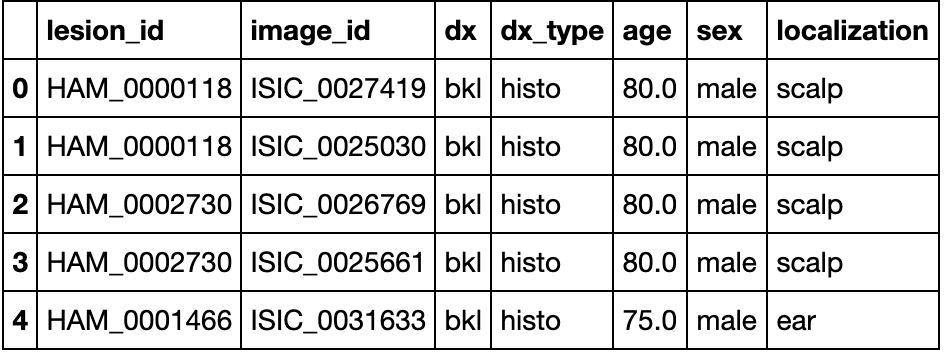
\includegraphics[width=\textwidth]{Images/datae.png}
    \caption{Pandas Dataframe containing information about pigmented skin lesions}
    \label{fig:pandasTop}
\end{figure}

The information was read using pandas into the data frame, 
which is a data structure that allows storing tabular data from CSV files as shown in 
figure \ref{fig:pandasTop} which represents the small section of the whole pandas dataframe. The CSV file contains irrelevant information such as age, sex and localisation 
of patients in the data frame which was removed by dropping the non essential columns.

\begin{figure} [!htp]
    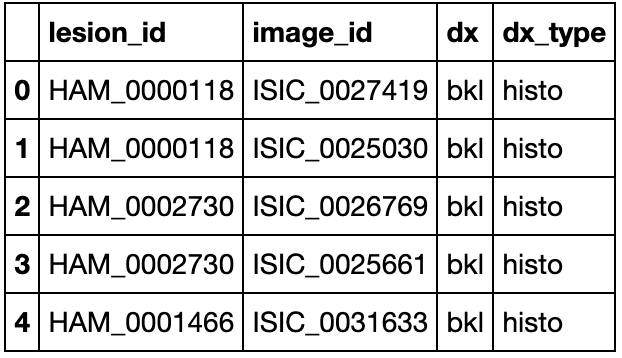
\includegraphics[width=\textwidth]{Images/datee.png}
    \caption{Pandas Dataframe containing essential information}
    \label{fig:pandasdrop}
\end{figure}

The figure \ref{fig:pandasdrop} represents the pandas essential columns as result of elemination of irrelevant information.
In addition, the dataset contains unclear and hairy images of pigmented skin lesions which were manually 
removed from the dataset to enhance the quality of available data.
Furthermore, the research only focuses on limited categories of 
pigmented skins which results in dropping data columns for the other categories 
of data. The information shown in \ref{fig:pandasdrop} dataframe contains a lesionid column which coresponds
to image names which were were read into numpy array using pillow library from respective directories.
The data for convolutional neural networks needs to divided into training and testing data, the model learnings
are peformed with learning the patterns and relationships in the training datasets and evaluation of the 
model is performed on the testing data which is never feed to the intelligent model which training.
The dataset was divided into training and testing sets using \url{sklearn.model_selection.train_test_split} class in the portion of 80 per cent for 
the training dataset and 20 per cent of testing datasets. The next step towards to preparing the dataset was reading the images data into NumPy 
array for both training and testing datasets and converting the image names from pandas series to NumPy array corresponding to each image and assign class number 
based on category of pigmented skin lesion in the dataset. Furthermore, the training and testing datasets were serialised into 
dictionary in a pickle encoded file. Therefore, the encoded file sizes are compact and are portable
in comparison to storing actual image files. \footnote{\url{https://github.coventry.ac.uk/sareenv/Final-Year-Project/blob/master/Research}}
\pagebreak